A consequence of separating physics and dynamics grids is that the atmospheric state must be mapped to the physics grid and the physics tendencies must be mapped back to the dynamics grid. Note that tendencies and not an updated state is mapped back to the dynamics grid. If one were to map an updated state the errors in the mapping process may adversely affect the simulation, e.g., in the case of no physics forcing there will be a non-zero `physics forcing' entirely due to the errors in the mapping algorithm.

In a climate model setting it is important that this process does not violate important conservation properties such as:
\begin{itemize}
\item mass-conservation,
\item shape-preserving (monotone), i.e. the mapping method does not introduce new extrema in the interpolated field, in particular, negatives,
\item consistency, i.e. the mapping preserves a constant.
\end{itemize}
Other properties that may be important, but not pursued here, is energy conservation and axial angular momentum conservation. It may be desirable to preserve the high-order of the basis functions during the mapping process so that the mapping is high-order accurate for smooth fields and less information is lost during the mapping process. 

{\color{red}{
\begin{itemize}
\item description of PHIS
\end{itemize}
}}
%\begin{equation}
%\psi=\phi_k\, \Delta p_k,
%\end{equation}
%where sub-script $k$ refers to the level index. [conversion back]
\subsection{Remapping state: GLL grid $\rightarrow$ physics grid}
The state variables that need to be mapped from the GLL grid to the physics grid are temperature $T^{(GLL)}$ and velocity components  $(u^{(GLL)},v^{(GLL)})$. Temperature is mapped by integrating the SE basis function representation of $T^{(GLL)}\times \Delta p^{(GLL)}$ and $\Delta p^{(GLL)}$ over the physics grid control volumes. The temperature on the physics grid is recovered from $\frac{T^{(phys)}\times \Delta p^{(phys)}}{\Delta\ p^{(phys)}}$. This mapping method conserves dry thermal energy $c_p^{(d)}T^{(GLL)}\times \Delta p^{(GLL)}$, where $c_p^{(d)}$ is the heat capacity for dry air at constant pressure, in each element. The velocity vectors are transformed from spherical coordinates to contravariant components \citep[see, e.g., section 3.2 in ][]{LetAl2017MWR} and the basis function representation of each contravariant velocity component is evaluated at the centerpoint of the physics grid control volumes. Thereafter the vectors are transformed back to spherical coordinates. Since the atmospheric state mapped from dynamics to physics grid is based on the high-order SE basis functions, the loss of accuracy in transferring the state from GLL to physics grid is minimized.


\begin{figure}[t]
\noindent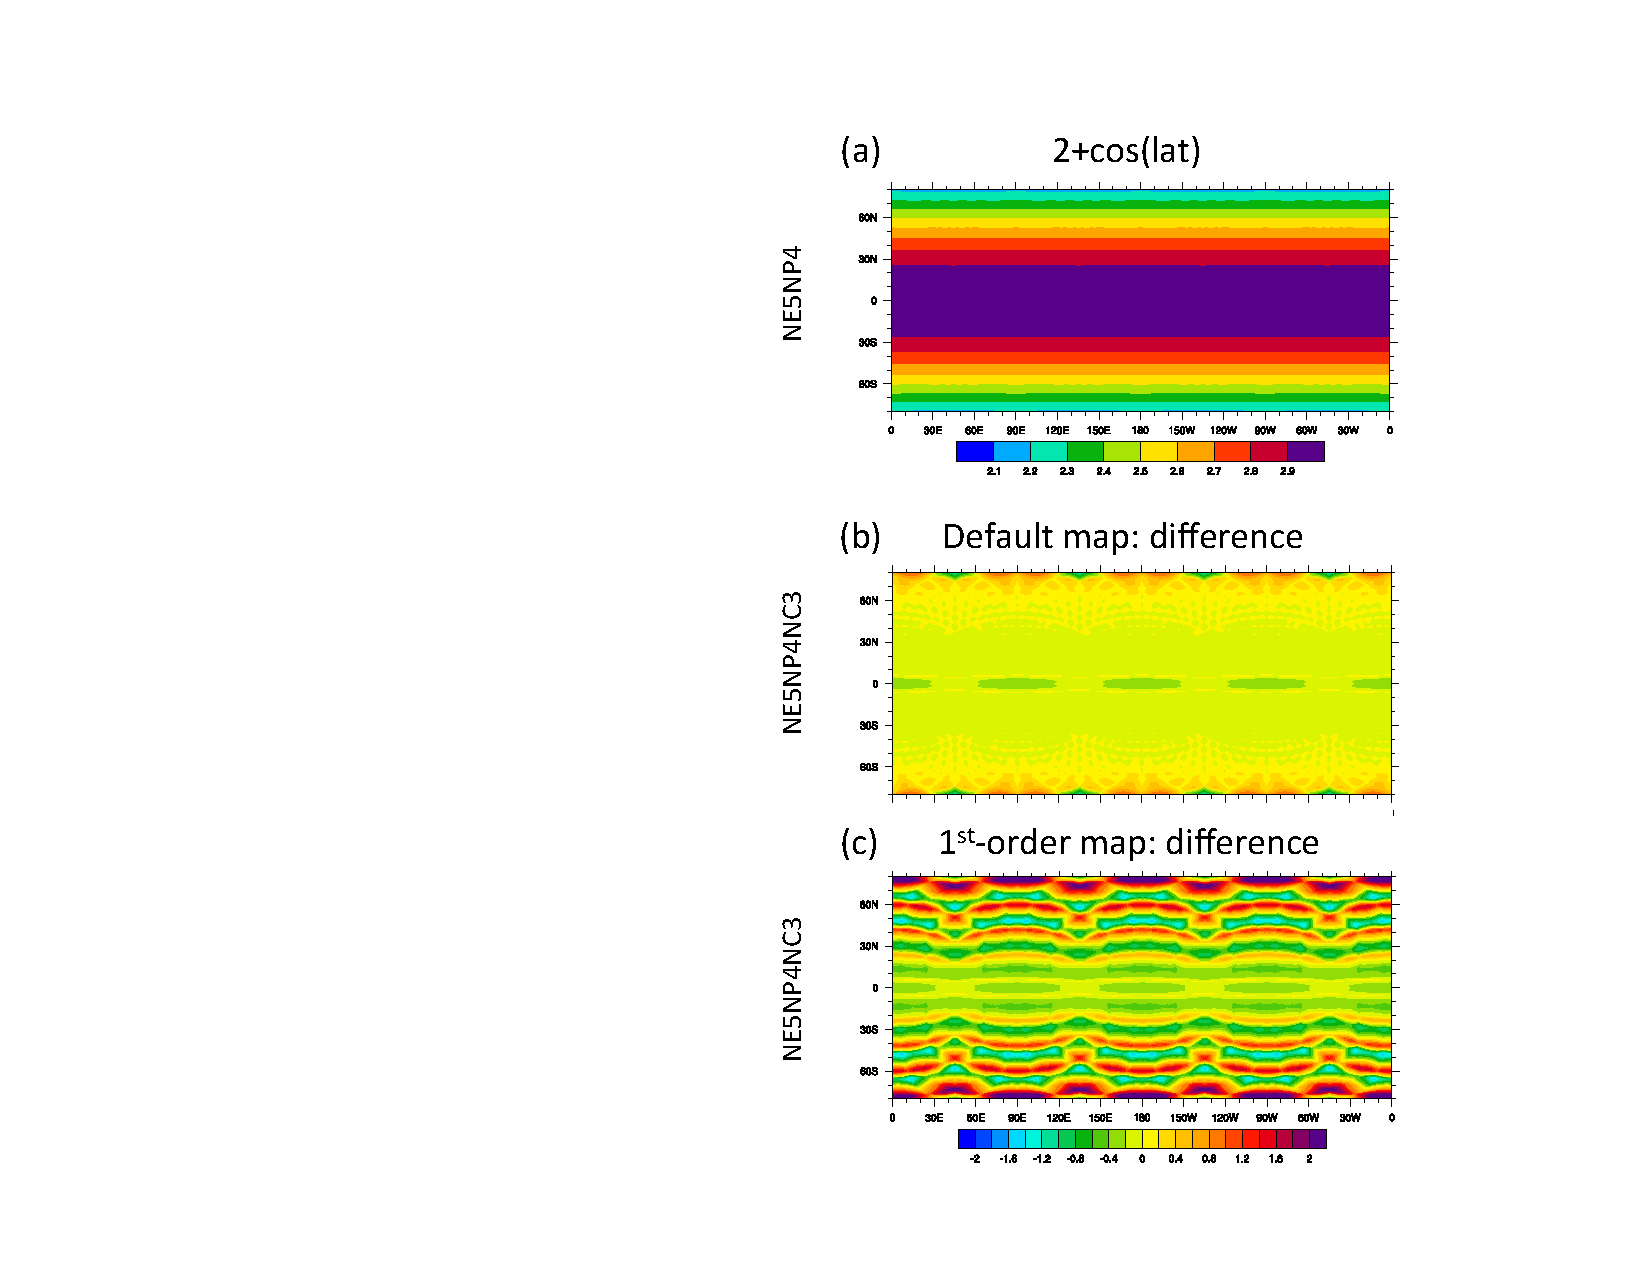
\includegraphics[width=19pc,angle=0]{figs/idealized-mapping-tests-smooth-field.pdf}\\
\caption{(a) Smooth function ($2+\cos(\theta)$) initialized on the $NE5NP4$ GLL grid. (b) and (c) show the difference between the interpolated field and the analytical value at the physics grid cell center. The interpolation is from the $NE5NP4$ GLL grid to the NE5NP4NC3 physics grid (both have an approximate grid spacing of $6^\circ$). In (b) the interpolation algorithm is the default algorithm that is higher-order for smooth fields, shape-preserving, consistent, and mass-conservative. (c) is the same as (b) but using the first-order mapping method. All data has been bilinearly interpolated to a $1^\circ$ regular latitude-longitude grid for plotting.}\label{fig:remap-smooth-field}
\end{figure}
\begin{figure}[t]
\noindent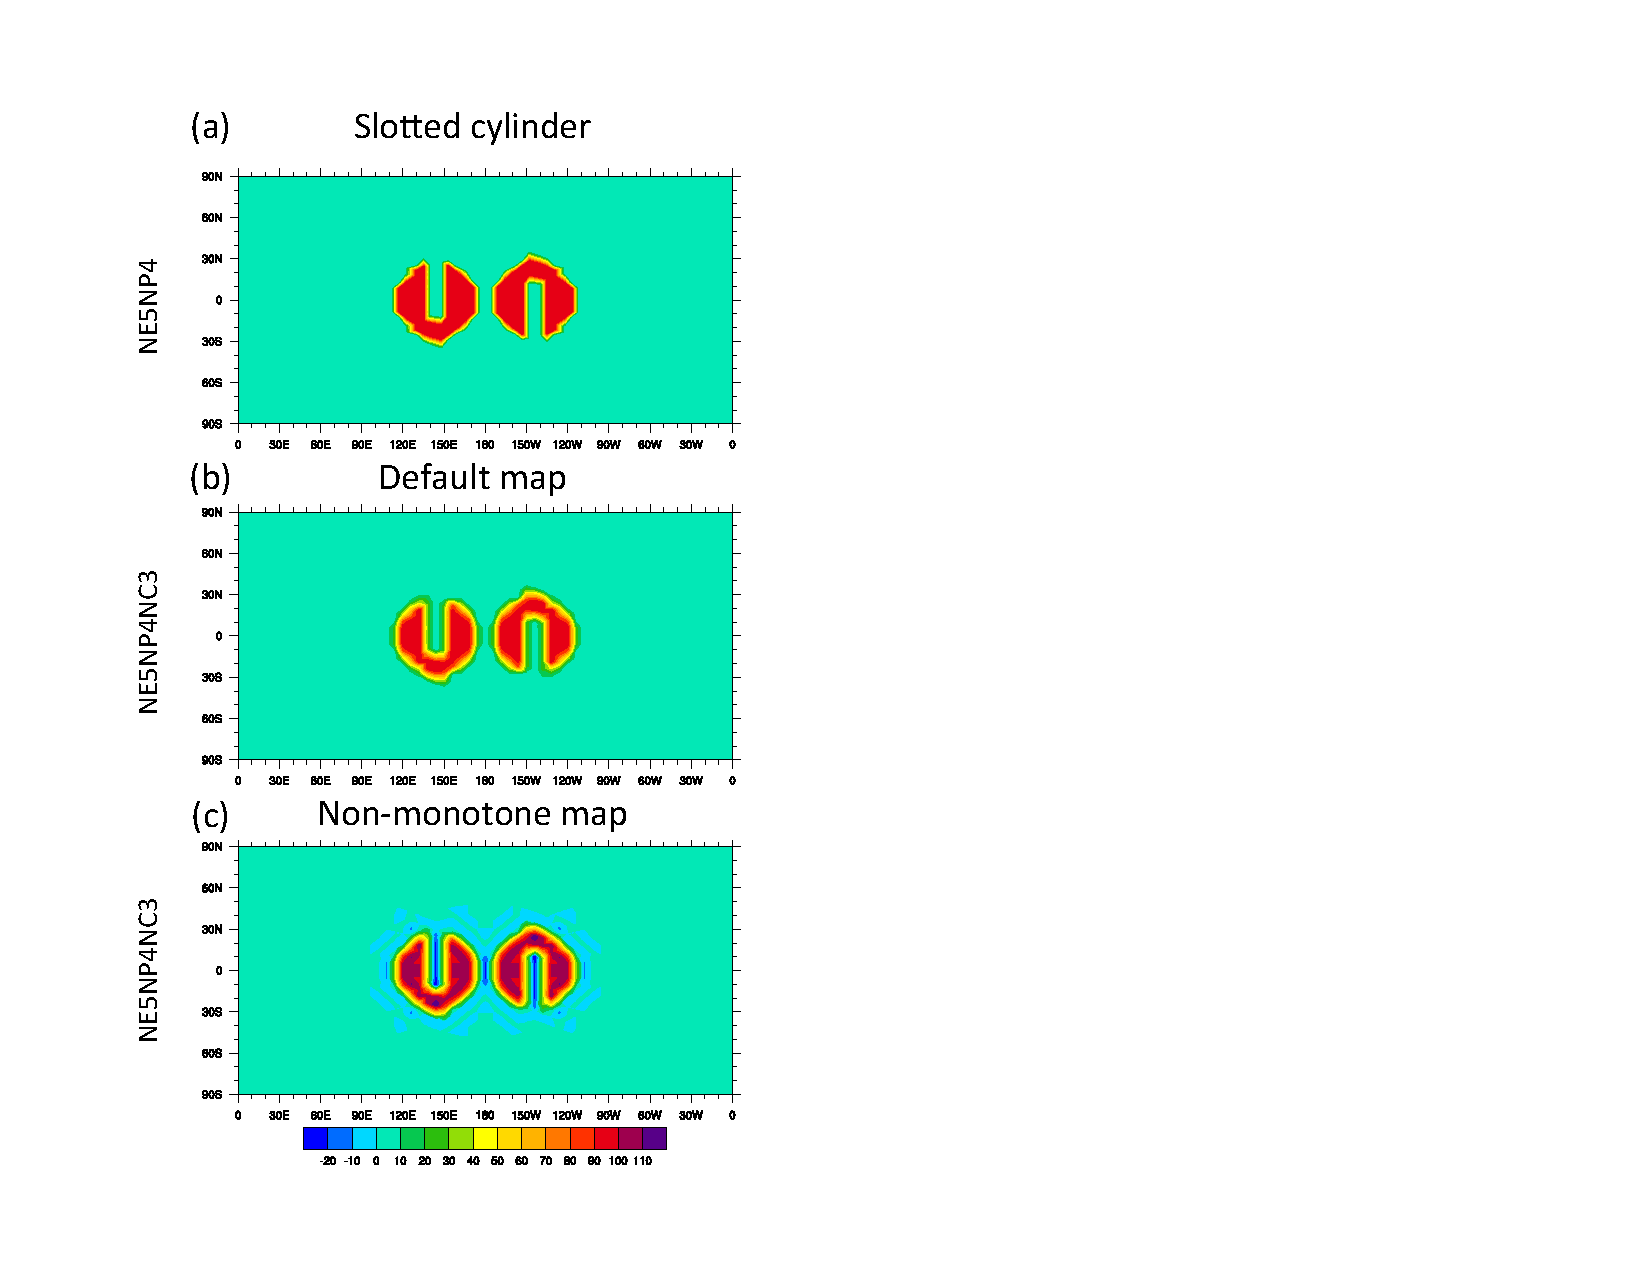
\includegraphics[width=19pc,angle=0]{figs/idealized-mapping-tests-slotted-cylinder.pdf}\\
  \caption{(a) Slotted-cylinder distribution initialized on on the $NE5NP4$ GLL grid (approximately $6^\circ$ resolution). (b) Default mapping of the $NE5NP4$ GLL grid data to the physics grid $NE5NP4NC3$. (c) Same as (b) but using the non-monotone map. All data has been bilinearly interpolated to a $1^\circ\
$ regular latitude-longitude grid for plotting.}\label{fig:remap-slotted-cylinder}
\end{figure}
 
%
%
\subsection{Remapping: physics grid $\rightarrow$ GLL grid}
The CAM physics package returns tendencies for temperature $f_T^{(phys)}$, velocity components $(f_u,f_v)^{(phys)}$, water vapor $f_Q^{(phys)}$, other tracers $f_q^{(phys)}$, and surface pressure $f_{PS}^{(phys)}$. The latter forcing is due to the vertical coordinate in CAM-SE being based on `wet' pressure (dry air mass plus the weight of water vapor) so if there is a change in moisture in the column then the `wet' surface pressure  $PS$ changes whereas the dry air mass (surface pressure) remains constant \citep[see section 3.1.8 `Adjustment of pressure to include change in mass of water vapor' in ][]{CAM5}. 

As for the dynamics to physics grid mapping, conservation is important and we therefore mass-weight the variables being mapped. For that $\Delta p$ on the physics and dynamics grid is needed. Mapping the updated surface pressure on the physics grid to the dynamics grid is not desirable: first of all, if there is no tendency on surface pressure then the mapped surface pressure on the GLL grid will be different from the surface pressure on the GLL grid before calling physics. As mentioned before, this is equivalent to having a spurious forcing on $PS$ entirely due to errors in the mapping algorithm. Secondly, conservation properties will result unless the GLL grid surface pressure is overwritten by the mapped $PS$ from the physics grid to the dynamics grid. To ensure conservation and spurious forcing due to mapping errors the following algorithm is adopted for the mass-weighting.

Let $\Delta p_{phys}$ be the updated pressure level thickness returned by physics. Map water-vapor mass $\Delta p_{phys}\, f_Q^{(phys)}$ from the physics to the dynamics grid using a conservative, consistent, and shape-preserving method (see below) resulting in $\Delta p_{phys}\, f_Q^{(phys)}$. This variable is the surface pressure tendency on the GLL grid, $f_{PS}^{(GLL)}$. Now take the surface pressure on the GLL grid before calling physics $p_s^{(GLL)}$ and add the surface pressure tendency $\Delta t PS^{(GLL)}$. This updated surface pressure $p_s^{(GLL)}$ defines the updated pressure-level thicknesses $\Delta p^{(GLL)}$. We use the physics updated pressure level thickness on the physics grid $\Delta p^{(phys)}$ for the mass-weighting of the physics tendencies $f^{(phys)}_i$, where $i=T$, $Q$, $q$, $u_x$. $u_y$, $u_z$, and $\Delta p^{(GLL)}$ for recovering the tendencies after mapping. The velocity forcing is transformed into a Cartesian coordinate system vector as for the dynamics to physics grid mapping.

\subsubsection{Mapping algorithm} [Paul: we are just using low-order map? would it be easy to switch to higher-order?] To build the non-monotone ``first guess'' map from the finite volume physics grid to the finite element dynamics grid, a continuous polynomial reconstruction of degree $n_c-1$ (and order $n_c$) is built that exactly interpolates the volume averaged values in each physics grid element.  For the monotone ``first guess'' map, a second-order bilinear reconstruction is instead employed that interpolates the density field at the center of each finite volume.  In each case the reconstruction is then sampled at each of the Gauss-Lobotto-Legendre nodes of the dynamics grid.

\section{Results}
\begin{figure}[t]
\noindent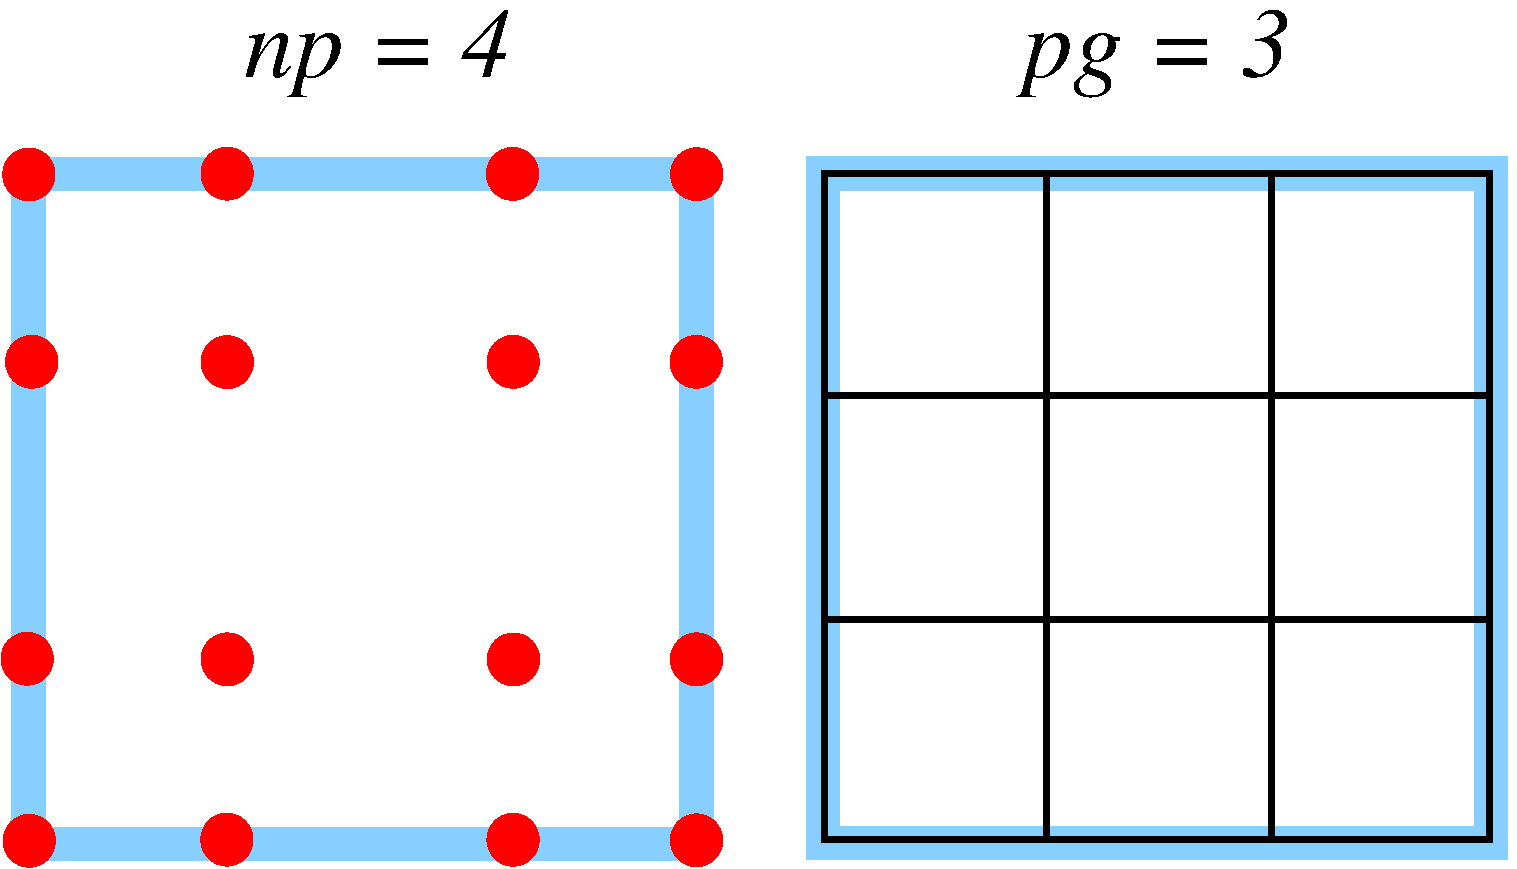
\includegraphics[width=19pc,angle=0]{figs/np4_pg3.pdf}\\
  \caption{A graphical illustration of the relationship between Gauss-Lobatto-Legendre quadrature grid for $np=4$ (left) and `equal-area' finite-volume grid with $pg=3$.}\label{fig:grids}
\end{figure}
%vs
